
\section{recommender algorithm}


\subsection{Information retrieval}
%%%%%%%%%%%%%%%%%%%%%%%%%%%%%%%%%
\iffalse
Was ist Information retrieval
in depth implementation is out of scope
Hinleitung zu Vektoren
\fi
%%%%%%%%%%%%%%%%%%%%%%%%%%%%%%%%%
\citeauthor{manning:2009} describe Information Retrieval in their book as process of "finding material [\dots] of an unstructured nature [\dots] that satisfies an information need from within a large collection."\citep[p.~1]{manning:2009}\\
In generall IR and RS are very similiar and a few technologies and findings of IR can be transfered to RS.
Since IR systems are build to handle unstructured data and transform them into a form that is easier to handle for computer systems one can adopt the method to RS input data such as items.\citep[p.~21-23]{ricci:2011}
There are various ways IR systems interpret data.
However this thesis will focus on one common method (and the theorie it depends on) called "tf-idf-vectors" which is a requirement for the Rocchio algorithm.\citep[p.~93]{lops:2011}\\
IR systems are built to handle "unstructured data".
Unstructured data is information bundled within a document (document is the IR related term for what is understood as item by RS) without any clear semantical structure.\citep[p.~1-3]{manning:2009}
The data within a document
IR systems can extract all relevant terms from a document
A term may resemble an attribute of an item such as its colour or brand.
The way of retrieving terms from a unstructured document is out of scope for this thesis but there is a brief example in figure~\ref{fig:TermRetrieving}.\\
For the section Information Retrieval the IR vocabulary will be adopted.
This means, that items will be called documents and attributes will be known as terms.

\begin{figure}[h]
    \center
    %\lstset{style=customHTML}
    \begin{lstlisting}
<html>
    <head><title>Online shop</title></head>
    <body>
        <img src="/img/p_42.jpg" alt="FancyBrand's product"/>
        <table>
            <tr><td>Colour</td><td>green</td></tr>
            <tr><td>Price</td><td>24,95 &euro;</td></tr>
            <tr><td>Brand</td><td>FancyBrand</td></tr>
        </table>
    </body>
</html>
    \end{lstlisting}
    \rowcolors{1}{\dustRowFirst}{\dustRowSecond}
    \begin{tabular}{ l }
        \rowcolor{\dustRowHead}
        \textbf{Terms:}\\\hline
        green\\
        24,95 \&euro;\\
        FancyBrand%\\\hline
    \end{tabular}
    \caption{Retrieving Terms from a HTML document.}
    \label{fig:TermRetrieving}
\end{figure}


\subsection{Weighting}
\label{sec:weighting}
As already mentioned a document can be be described as a collection of terms.
The process of locating terms within a document is taken for granted.
When a user queries for a specific term one has to find each relevant document including this term.
Also an order regarding the documents significance will be required.
The terms significance within a document is defined by its weight.\citep[p.~117]{manning:2009}\\
While primitive IR methods such as boolean retrieval only check for the existance of a queried term within a document weighting can give more precise results regarding the terms significance in a document.\citep[p.~109]{manning:2009}

\paragraph{Term frequency}
\label{sec:tf}
\index{Term Frequency}
A simple method to quantify the importance of a term within a document is the so called term frequency.
The concept is based on the assumption that the frequency of a term $t$ indicates its importance within a document $d$.
It is denoted as $\text{tf}_{t,d}$ where $t$ resembles the term an $d$ the document.
The number of occurences of $t$ within $d$ can be directly interpreted its term frequency.\citep[p.~117]{manning:2009}\\
For products of an online shop and its resulting term frequency may look like as described in figure~\ref{fig:tfweighting}.\\
\begin{figure}[h]

    \begin{quote}
        Document $\text{d}1$ with identified terms underlined:\\
        \underline{blouse} \underline{blue} \underline{55} Euro. \underline{55} cm by size \underline{S}. 100\% \underline{Polyester}
    \end{quote}

    \center
    \vspace{5mm}
    \rowcolors{0}{\dustRowFirst}{\dustRowSecond}
    \begin{tabular}{ l l }
        \rowcolor{\dustRowHead}
        \multicolumn{2}{c}{Term frequency}\\\hline
        $\text{tf}_{\text{blouse},\text{d1}}$       & 1\\
        $\text{tf}_{\text{blue},\text{d1}}$         & 1\\
        $\text{tf}_{\text{55},\text{d1}}$           & 2\\
        $\text{tf}_{\text{S},\text{d1}}$            & 1\\
        $\text{tf}_{\text{Polyester},\text{d1}}$    & 1\\
    \end{tabular}

    \caption{Term frequency weighting}
    \label{fig:tfweighting}
\end{figure}

\paragraph{Inverse document frequency}
\label{sec:idf}
\index{Inverse Document Frequency}
In some domains special terms will often appear multiple times within a document and therefore have high term frequency weight without giving any explanatory value.\citep[p.~117]{manning:2009}
Documents resembling clothing offered by an online shop may always include the name of the store as term.
Since the user already explicitely searches on the store, the relevance of this term is rather low.
In order to transfer this to weighting, inverse document weighting (idf) has been implemented.
Idf will scale down the weighting of terms that appear in all documents.
To do so, an intermediate step is neccessary. Before calculating the idf for a term one has to determine both the terms document frequency ($\text{df}_t$) and the total count of documents (as $N$).
Next the idf can be calculated with following forumla:\citep[p.~117-118]{manning:2009}\\
\begin{equation}
    \text{idf}_{t} = \log\frac{N}{\text{df}_{t}}
    \label{eq:idf-forumula}
\end{equation}
The logarithms basis isn't of great importance.\citep[p.~118]{manning:2009}
The examples however use 10 as base.
A more explanatory example is presented by figure~\ref{fig:idfweighting}.
The example states that rare items posses a higher idf, whereas more frequent terms are rated lower.\citep[p.~118]{manning:2009}\\
\begin{figure}[h]
    \begin{quote}
        Total count of documents  $N$ is 500\\
        Term1 "FancyShop" appears in 500 documents\\
        Term2 "blouse" appears in 130 documents\\
    \end{quote}

    \center
    \begin{tabular}{ l | l }
        $\text{df}_{\text{FancyShop}} = 500$                                                                    & $\text{df}_{\text{blouse}} = 130$\\
        $\text{idf}_{\text{FancyShop}} = \log\frac{N}{\text{df}_{\text{FancyShop}}} = \log\frac{500}{500} = 0$  & $\text{idf}_{\text{blouse}} = \log\frac{N}{\text{df}_{\text{blouse}}} = \log\frac{500}{130} \approx 0.59$
    \end{tabular}

    \caption{Inverse document frequency weighting}
    \label{fig:idfweighting}
\end{figure}

\paragraph{Tf-Idf}
\label{sec:tfidf}
\index{TfIdf}
Both the term frequency, as well as the inverse document frequency have some drawbacks.
While term frequency may weight terms with little informative value high because they appear often, inverse document frequency can totally ignore them by weighting them extremely low.
But it's possible to combine td and idf in order to get better weightings.
The result is called tf-idf.\citep[p.~118-119]{manning:2009}
\begin{equation}
    \text{tf-idf}_{\text{t,d}} = \text{tf}_\text{t,d} \times \text{idf}_\text{d}
    \label{eq:tf-idf-forumula}
\end{equation}

\noindent
Figure~\ref{fig:tfidfweighting} illustrates the generation of an tf-idf weighting.
\begin{figure}[h]

    \begin{quote}
        Total number of documents $N$ is 3\\
    \end{quote}

    \center
    \rowcolors{1}{\dustRowFirst}{\dustRowSecond}
    \begin{tabular}{ l l | l l l l }
        \rowcolor{\dustRowHead}
        Term                    & Document          & tf    & df & idf   & tf-idf\\\hline
        blouse                  & $\text{doc}_1$    & 15    &  2 & 0.18  & 2.7\\
        blouse                  & $\text{doc}_2$    & 5     &  2 & 0.18  & 0.9\\
        blouse                  & $\text{doc}_3$    & 9     &  2 & 0.18  & 1.62\\
    \end{tabular}
    \caption{tf-idf weighting}
    \label{fig:tfidfweighting}
\end{figure}

\noindent
\citeauthor{manning:2009} describes tf-idf weighting as follows:\\
"$\text{[Tf-idf}_{\text{t,d}}\text{]}$ assigns to term $t$ a weight in document $d$ that is
\begin{enumerate}
    \item highest when $t$ occurs many times within a small number of documents
    (thus lending high discriminating power to those documents);
    \item lower when the term occurs fewer times in a document, or occurs in many
    documents (thus offering a less pronounced relevance signal);
    \item lowest when the term occurs in virtually all documents."
\end{enumerate}
\citep[p.~119]{manning:2009}

\subsubsection{Vector space model}
\label{sec:vectorspacemodel}
\index{VectorSpaceModel}
Any document can now be described as a vector.
Each term in a document will be directly interpreted as component of a vector.
If a term is non existent in a document, the vector component will be numeric zero.\citep[p.~120]{manning:2009}\\
Therefore IR provids methods to describe documents as vectors.
Forging a bridge back to RS the vectors can help to provide a computer representation of real world products.
The vectors of all products can be displayed in one common vector space.
This process is known as vector space model.\citep[p.~120]{manning:2009}
An example of a two dimensional vector space model is given in figure~\ref{fig:vectorspacemodel}.


\begin{figure}[h]

    \begin{quote}
        There are three documents with following terms:\\
        Document $\text{d}_1$: $1\times \text{FancyBrand}, 2\times \text{green}$\\
        Document $\text{d}_2$: $1\times \text{FancyBrand}$\\
        Document $\text{d}_3$: $1\times \text{green}$\\
        Whereas "FancyBrand" and "green" are the document terms.

        \noindent
        The generic tf-idf vector representation of one of the documents above will be:\\
        $\vec{\text{v}}_{\text{generic}} = (\text{tf-idf}_{\text{FancyBrand},\text{d}_\text{generic}}, \text{tf-idf}_{\text{green},\text{d}_\text{generic}})^T$

        \noindent
        The corresponding tf-idf-vectors of the are:\\
        $\vec{\text{v}}_1 = (\text{tf-idf}_{\text{FancyBrand},\text{d}_1}, \text{tf-idf}_{\text{green},\text{d}_1})^T = (0.18, 0.35)^T$\\
        $\vec{\text{v}}_2 = (\text{tf-idf}_{\text{FancyBrand},\text{d}_2}, \text{tf-idf}_{\text{green},\text{d}_2})^T = (0.18, 0)^T$\\
        $\vec{\text{v}}_3 = (\text{tf-idf}_{\text{FancyBrand},\text{d}_3}, \text{tf-idf}_{\text{green},\text{d}_3})^T = (0, 0.18)^T$\\
    \end{quote}

    \center
    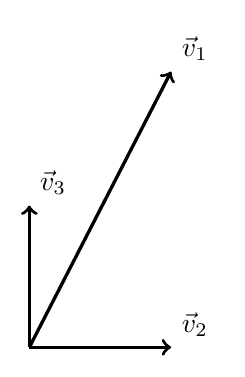
\begin{tikzpicture}
        \tkzInit[xmax=0.5,ymax=0.5,xstep=0.1,ystep=0.1]
        %\tkzAxeX[label=FancyBrand,above left=10pt]
        \tkzAxeX[label=FancyBrand, right]
        %\tkzAxeY[label=green,below right=30pt]
        \tkzAxeY[label=green,above]
        \tkzGrid
        \draw[very thick, ->] (0,0) -- (1.8,3.5) node[anchor=south west]{$\vec{\text{v}}_1$};
        \draw[very thick,latex-latex, ->] (0,0) -- (1.8,0) node[anchor=south west]{$\vec{\text{v}}_2$};
        \draw[very thick,latex-latex, ->] (0,0) -- (0, 1.8) node[anchor=south west]{$\vec{\text{v}}_3$};
    \end{tikzpicture}

    \caption{Two dimensional vector space model}
    \label{fig:vectorspacemodel}
\end{figure}


\subsubsection{Parametric and zone indices}
\label{sec:parametricandzoneindices}

% evtl. noch ausf\"uhren:
% - stop words (woerter die nicht gewertet werden z.b. ist, er war, ...)
% - Parametric and zones indices


\subsection{Rocchio's algorithm}
\label{sec:rocchio}
%%%%%%%%%%%%%%%%%%%%%%%%%%%%%%%%%%%%
\iffalse
Beschreibung des Rocchio algorithmus
\fi
%%%%%%%%%%%%%%%%%%%%%%%%%%%%%%%%%%%%
With section~\ref{sec:tfidf} and section~\ref{sec:vectorspacemodel} the requirements of Rocchio's algorithm have been described.\citep[p.~178]{manning:2009}
The next step is to specify the algorithm itself.
{\color{red} Kommt eigentlich aus information retrieval und hilft dabei items zu finden.
Bietet also vorschlaege zu einer suchanfrage, wobei die anfrage die bisher gewaehlten producte sind.}
Rocchio's relevance feedback algorithm is classified as content-based RS.\citep[p.~92]{lops:2011}
The algorithm tries to find a vector representing the user that is similiar to all item which are relevant to the user.
In addition the number of unrelevant item matching the vector should be minimal.\citep[p.~178-181]{manning:2009}
One of the algorithms charakteristics is the way feedback (as described in section~\ref{sec:feedback}) is treated.
Every time the user gives either positive or negative feedback, the algorithm will adapt the user vector to match the new criteria.\citep[p.~387-388]{pazzani:2007}
\\

When using Rocchio's algorithm for a recommender system one uses a user vector instead of a query vector as originally intended.
\begin{equation}
    \vec{\text{q}}_m =
        \alpha \cdot \vec{\text{q}}_0
        + \beta \cdot \frac{1}{|\text{D}_\text{r}|}\sum_{\vec{\text{d}}_j\in \text{D}_\text{r}} \vec{\text{d}}_j
        - \gamma \cdot \frac{1}{|\text{D}_\text{nr}|}\sum_{\vec{\text{d}}_j\in \text{D}_\text{nr}} \vec{\text{d}}_j
\end{equation}
$\vec{\text{q}}_0$ is the old vector representing the user before he gave feedback about one of the items.
The result $\vec{\text{q}}_m$ however is the modified vector describing the user after his most recent feedback has been considered.
For each calculation with Rocchio's algorithm $\vec{\text{q}}_0$ will always be the result $\vec{\text{q}}_m$ of the preceding calculation.\\
$\text{D}_\text{r}$ is a set of all relevant item vectors, while $\text{D}_\text{nr}$ represents a set of items that are unrelevant to the user.\\
$\alpha$, $\beta$ and $\gamma$ act as weights and can influence the importance of the old user vector, as well as of  the relevant and unrelevant documents.
The old user vector is weighted by $\alpha$.
The average of relevant documents is weighted by $\beta$ and $\gamma$ is responsible for unrelevant documents.
There are only positive values for weights allowed.
The lowest possible weight is 0.
A well established configuration for these weights is: $\alpha = 1$, $\beta = 0.75$ and $\gamma = 0.15$.
However if a RS only allows positive feedback, one can as well set $\gamma$ to 0.
\citep[p.~178-183]{manning:2009}
